\section{Projected Bellman Error}
\label{sec:bellman_error}

This section explains several key ideas in Reinforcement Learning and Approximate Dynamic Programming:


In approximate dynamic programming or reinforcement learning, $v$ may lie in a restricted function space (e.g., a parametric class of value functions). Hence, we cannot always solve exactly.
\[
(I - P)\,\boldsymbol{v} = \boldsymbol{r} - g\,\mathbf{1}
\]
\noindent
where:
\begin{itemize}
    \item $\boldsymbol{v}$ is the vector of values $v(s)$,
    \item $\boldsymbol{r}$ is the vector of immediate rewards $r(s)$,
    \item $\mathbf{1}$ is a vector of all ones,
    \item $P$ is a state-transition matrix (or its expectation under the policy), so that $P'\boldsymbol{v}$ corresponds to $\mathbb{E}[v(s')]$.
\end{itemize}

Instead, we use a \emph{projection} operator $\mathbb{P}$ that projects any function onto our approximation space. Thus, the \emph{projected Bellman error} (PBE) is defined as:
\[
\text{PBE}(v) 
\;=\; \mathbb{P}\Bigl[(r - g\,\mathbf{1}) + P\,v\Bigr] \;-\; v.
\]
This quantity indicates how close the projected Bellman update $\mathbb{P}[\mathbb{B}v]$ is to $v$, where the Bellman operator is given by
\[
\mathbb{B}v \;\equiv\; r - g\,\mathbf{1} \;+\; Pv.
\]
Minimizing the PBE is a common strategy in methods such as LSTD, where we seek a parameterized value function $\hat{v}(w)$ that is as close as possible (in a projected sense) to the Bellman update.

\subsubsection{Norm-Based View of PBE}
A common way to quantify the PBE is via a weighted $\ell_2$-norm (often using the stationary distribution $p^*(s)$ as weights). Let
\[
\Delta v(s) \;=\; \hat{v}(w)(s) \;-\; \mathbb{P}\bigl[\mathbb{B}\,\hat{v}(w)\bigr](s).
\]
Then, the PBE can be measured as:
\[
e_{\mathrm{PB}}
\;=\;
\bigl\lVert \Delta v \bigr\rVert_{p^*}^2
\;=\;
\sum_{s} p^*(s)\,\bigl[\Delta v(s)\bigr]^2
\;=\;
\mathbb{E}_{s \sim p^*}\bigl[\Delta v(s)^2\bigr].
\]
When $e_{\mathrm{PB}} = 0$, it implies that $\hat{v}(w)$ is a fixed point of the projected Bellman operator, i.e., $\hat{v}(w) = \mathbb{P}[\mathbb{B}\,\hat{v}(w)]$.

\subsection{Why It Does Not Involve the True Value}
A key point is that we do \emph{not} need the \emph{true} value function $v^*$ to measure or minimize the Bellman error equation (or the projected Bellman error). Instead, we only need:
\begin{itemize}
    \item Observations of $(s, r(s), s')$ transitions (in model-free settings), or
    \item A model for the reward and transition probabilities (in model-based settings).
\end{itemize}
From these, we can construct the Bellman operator $\mathbb{B}$ (or an empirical version of it) and compare $\mathbb{B}v$ to $v$. This approach is stable because it relies on the \emph{self-consistency} property of the Bellman equation rather than on direct knowledge of $v^*$.

\subsection{Temporal Difference Error Connection}
Methods like \emph{Temporal Difference (TD) learning} effectively estimate the Bellman error equation incrementally. A TD update can be viewed as trying to drive the quantity
\[
\delta_t 
= r_t - g + v(s_{t+1}) - v(s_t)
\]
to zero over time, which corresponds to making $v$ satisfy the Bellman equation in expectation.

\subsection{Geometric Interpretation in Parameter Space}

\begin{figure}[ht]
    \centering
    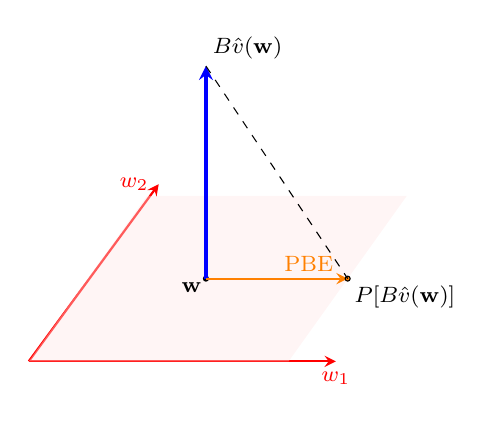
\begin{tikzpicture}[scale=3, x={(1cm,0cm)}, y={(0.5cm,0.5cm)}, z={(0cm,1cm)}, >=stealth]
    
        % Axes
        \draw[->, thick, red] (0,0,0) -- (1.3,0,0) node[below] {\footnotesize $\boldsymbol{w}_1$};
        \draw[->, thick, red] (0,0,0) -- (0,1.1,0.2) node[left] {\footnotesize $\boldsymbol{w}_2$};
    
        % Tilted parameter plane
        \fill[red!10, opacity=0.4] (0,0,0) -- (1.1,0,0) -- (1.1,1,0.2) -- (0,1,0.2) -- cycle;
    
        % Point w
        \coordinate (Wbase) at (0.5,0.5,0.1);
        \node[below left=-2pt] at (Wbase) {\footnotesize $\mathbf{w}$};
        \draw[fill=black] (Wbase) circle (0.3pt);
    
        % Bellman update vector (blue)
        \coordinate (Bv) at (0.5,0.5,1.0);
        \draw[->, very thick, blue] (Wbase) -- (Bv);
        \node[above right=-1pt] at (Bv) {\footnotesize $\mathbb{B}\hat{v}(\mathbf{w})$};
    
        % Projection of Bellman update (PBE) on plane
        \coordinate (Proj) at (1.1,0.5,0.1);
        \draw[->, thick, orange] (Wbase) -- (Proj) node[midway, above right=-1pt] {\footnotesize \textcolor{orange}{PBE}};
        
        % Tip of projection labeled as P[Bv]
        \draw[fill=orange] (Proj) circle (0.3pt);
        \node[below right=-1pt] at (Proj) {\footnotesize $\mathbb{P}[\mathbb{B}\hat{v}(\mathbf{w})]$};
    
        % Optional dashed helper from blue tip to projection
        \draw[dashed] (Bv) -- (Proj);
    
    \end{tikzpicture}
    \caption{The Bellman update $\mathbb{B}\hat{v}(\mathbf{w})$ (blue) lifts from the point $\mathbf{w}$ in parameter space. Its projection $\mathbb{P}[\mathbb{B}\hat{v}(\mathbf{w})]$ lies within the tilted space defined by $\boldsymbol{w}_1$ and $\boldsymbol{w}_2$, and the Projected Bellman Error (PBE, orange) spans between them.}
    \label{fig:bellman-final}
    \end{figure}

\paragraph{Explanation of the Diagram:}
\begin{itemize}
    \item \textbf{Parameter Space:} The light red square represents the 2D parameter space, with axes $w_1$ and $w_2$. Every point in this space corresponds to a set of parameters $\mathbf{w}$ defining the approximate value function $\hat{v}(\mathbf{w})$.
    \item \textbf{Current Parameter Vector:} The point labeled $\mathbf{w}$ (located at $(1,1)$ in this example) is our current estimate in the parameter space.
    \item \textbf{Bellman Operator Application:} The arrow from $\mathbf{w}$ to the point labeled $\mathbb{B}\hat{v}(\mathbf{w})$ represents the application of the Bellman operator. This update may move the value function outside the representable parameter space.
    \item \textbf{Projection Operator:} The dashed line and the point $\mathbb{P}[\mathbb{B}\hat{v}(\mathbf{w})]$ indicate that we use a projection operator $\mathbb{P}$ to map the Bellman update back into our parameter space.
    \item \textbf{Projected Bellman Error (PBE):} The orange arrow from $\mathbf{w}$ to $\mathbb{P}[\mathbb{B}\hat{v}(\mathbf{w})]$ represents the Projected Bellman Error. Minimizing this error is key to ensuring that our approximate value function is as close as possible to being a fixed point of the projected Bellman operator.
\end{itemize}

\subsection{Projection Operator \texorpdfstring{$\mathbb{P}$}{P}}

Suppose we have:
\[
\text{feature matrix: } F \in \mathbb{R}^{|S|\times k}, 
\quad
\text{diagonal weighting: } D_{p^*} \in \mathbb{R}^{|S|\times |S|}.
\]
Here, $|S|$ is the number of states (or samples), and each row of $F$ is a feature vector $\boldsymbol{f}(s)^T$ for state $s$. The matrix $D_{p^*}$ is diagonal with entries $p^*(s)$, representing a stationary distribution or weighting over states.

We wish to define a \emph{projection} operator
\[
\mathbb{P}: \mathbb{R}^{|S|} \;\to\; \text{Col}(F),
\]
where $\text{Col}(F)$ is the column space spanned by $F$. The projection is taken under the $\ell_2$-norm weighted by $D_{p^*}$, namely
\[
\|\boldsymbol{x}\|_{D_{p^*}}^2 \;=\; \boldsymbol{x}^T\,D_{p^*}\,\boldsymbol{x}.
\]
Formally, for any vector $\boldsymbol{v} \in \mathbb{R}^{|S|}$, we define
\[
\mathbb{P}(\boldsymbol{v}) \;=\; \arg\min_{\boldsymbol{x} \in \text{Col}(F)} \;\|\boldsymbol{v} - \boldsymbol{x}\|_{D_{p^*}}^2.
\]
Since $\boldsymbol{x} \in \text{Col}(F)$ can be written as $\boldsymbol{x} = F\boldsymbol{w}$ for some $\boldsymbol{w} \in \mathbb{R}^k$, the problem becomes:
\[
\mathbb{P}(\boldsymbol{v}) 
\;=\; \arg\min_{F\boldsymbol{w}} \;\|\boldsymbol{v} - F\boldsymbol{w}\|_{D_{p^*}}^2.
\]
We can solve for $\boldsymbol{w}$ by expanding and taking derivatives.

\paragraph{Step-by-Step Derivation:}

\begin{enumerate}
    \item \textbf{Rewrite the objective:}
    \[
    \|\boldsymbol{v} - F\boldsymbol{w}\|_{D_{p^*}}^2 
    \;=\; (\boldsymbol{v} - F\boldsymbol{w})^T\,D_{p^*}\,(\boldsymbol{v} - F\boldsymbol{w}).
    \]
    
    \item \textbf{Take the gradient with respect to $\boldsymbol{w}$:}
    \[
    \frac{\partial}{\partial \boldsymbol{w}} 
    \bigl[(\boldsymbol{v} - F\boldsymbol{w})^T\,D_{p^*}\,(\boldsymbol{v} - F\boldsymbol{w})\bigr]
    \;=\;
    -2\,F^T\,D_{p^*}\,(\boldsymbol{v} - F\boldsymbol{w}).
    \]
    Setting this to zero for optimality yields:
    \[
    F^T\,D_{p^*}\,(\boldsymbol{v} - F\boldsymbol{w}) \;=\; 0 
    \quad\Longrightarrow\quad
    F^T\,D_{p^*}\,F\,\boldsymbol{w} \;=\; F^T\,D_{p^*}\,\boldsymbol{v}.
    \]
    
    \item \textbf{Solve for $\boldsymbol{w}$:}
    \[
    \boldsymbol{w}^* 
    \;=\; \bigl(F^T\,D_{p^*}\,F\bigr)^{-1}\,F^T\,D_{p^*}\,\boldsymbol{v}.
    \]
    
    \item \textbf{Hence, the projection of $\boldsymbol{v}$:}
    \[
    \mathbb{P}(\boldsymbol{v})
    \;=\; F\,\boldsymbol{w}^*
    \;=\; F\,\bigl(F^T\,D_{p^*}\,F\bigr)^{-1}\,F^T\,D_{p^*}\,\boldsymbol{v}.
    \]
\end{enumerate}
As introduced by \cite{bradtke1996least}, the LSTD algorithm projects the Bellman operator into the function space.

Therefore, the projection operator $\mathbb{P}$ onto the column space of $F$ under the $D_{p^*}$-weighted norm is
\[
\boxed{
\mathbb{P} 
\;=\; 
F\,\bigl(F^T\,D_{p^*}\,F\bigr)^{-1}\,F^T\,D_{p^*}.
}
\]
In other words, for any vector $\boldsymbol{v}$, $\mathbb{P}(\boldsymbol{v})$ is given by the above formula.


\subsection{Deriving \texorpdfstring{$\boldsymbol{w}^*$}{w*} to Minimize the Projected Bellman Error}

Next, consider a \emph{linear} approximate value function:
\[
\hat{v}(\boldsymbol{w}) \;=\; F\,\boldsymbol{w}.
\]
The \emph{Projected Bellman Error} (PBE) can be defined (in squared norm) as
\[
e_{\mathrm{PB}}(\boldsymbol{w})
\;=\;
\bigl\|
\hat{v}(\boldsymbol{w}) 
\;-\;
\mathbb{P}\bigl[\mathbb{B}\,\hat{v}(\boldsymbol{w})\bigr]
\bigr\|_{D_{p^*}}^2,
\]
where $\mathbb{B}$ is the Bellman operator, e.g.,
\[
\mathbb{B}\,\hat{v}(\boldsymbol{w})
\;=\;
\boldsymbol{r} \;-\; g\,\mathbf{1}
\;+\;
P\,\bigl(F\,\boldsymbol{w}\bigr).
\]
We want:
\[
\boldsymbol{w}^*
\;=\;
\arg\min_{\boldsymbol{w}}
\;e_{\mathrm{PB}}(\boldsymbol{w}).
\]

\paragraph{Outline of the Solution:}
\begin{itemize}
    \item \textbf{Apply $\mathbb{P}$:} 
    \[
    \mathbb{P}\bigl[\mathbb{B}\,\hat{v}(\boldsymbol{w})\bigr]
    \;=\;
    F\,(F^T D_{p^*} F)^{-1} F^T\,D_{p^*}\,\bigl(\boldsymbol{r} - g\,\mathbf{1} + P\,F\,\boldsymbol{w}\bigr).
    \]
    
    \item \textbf{Compute the difference:}
    \[
    \hat{v}(\boldsymbol{w}) 
    \;-\;
    \mathbb{P}\bigl[\mathbb{B}\,\hat{v}(\boldsymbol{w})\bigr]
    \;=\;
    F\,\boldsymbol{w}
    \;-\;
    F\,(F^T D_{p^*} F)^{-1} F^T\,D_{p^*}\,\bigl(\boldsymbol{r} - g\,\mathbf{1} + P\,F\,\boldsymbol{w}\bigr).
    \]
    
    \item \textbf{Square under $D_{p^*}$:}
    \[
    e_{\mathrm{PB}}(\boldsymbol{w})
    \;=\;
    \bigl\|
    F\,\boldsymbol{w}
    \;-\;
    F\,(F^T D_{p^*} F)^{-1} F^T\,D_{p^*}\,\bigl(\boldsymbol{r} - g\,\mathbf{1} + P\,F\,\boldsymbol{w}\bigr)
    \bigr\|_{D_{p^*}}^2.
    \]
    One can then take the gradient with respect to $\boldsymbol{w}$ and set it to zero. 
    Under suitable assumptions (like invertibility of $(F^T D_{p^*} (I - P) F)$), 
    the resulting $\boldsymbol{w}^*$ often matches the well-known LSTD solution:
    \[
    \boldsymbol{w}^*
    \;=\;
    \bigl(F^T\,D_{p^*}\,\bigl(I - P\bigr)\,F\bigr)^{-1}
    F^T\,D_{p^*}\,\bigl(\boldsymbol{r} - g\,\mathbf{1}\bigr).
    \]
\end{itemize}

\paragraph{Interpretation.}
\begin{itemize}
    \item \emph{Projection}: We only need to operate in the subspace spanned by $F$. Instead of trying to match the Bellman operator $\mathbb{B}\hat{v}(\boldsymbol{w})$ exactly, we \emph{project} it back into $\text{Col}(F)$.
    \item \emph{Weighted Norm}: The diagonal matrix $D_{p^*}$ imposes a weighting, typically corresponding to a stationary distribution over states. States with higher probability mass get higher influence in the error measure.
    \item \emph{Minimizing PBE}: Solving $\arg\min_{\boldsymbol{w}} e_{\mathrm{PB}}(\boldsymbol{w})$ yields $\boldsymbol{w}^*$ that best satisfies the Bellman equation in the projected sense. This is precisely the principle behind LSTD and related least-squares policy/value evaluation methods.
\end{itemize}

\noindent
\textbf{Final Summary.}  
The key formulas are:
\[
\boxed{
\mathbb{P}(\boldsymbol{v}) 
= 
F \,\bigl(F^T\,D_{p^*}\,F\bigr)^{-1}\,F^T\,D_{p^*}\,\boldsymbol{v},
\quad
\boldsymbol{w}^*
= 
\arg\min_{\boldsymbol{w}}\,
\bigl\|\,
F \boldsymbol{w}
\;-\;
\mathbb{P}\bigl[\mathbb{B}(F \boldsymbol{w})\bigr]
\bigr\|_{D_{p^*}}^2.
}
\]
They show how the projection operator arises from a simple least-squares argument and how, in turn, one can derive the optimal parameter vector $\boldsymbol{w}^*$ by minimizing the Projected Bellman Error.

\subsection{Taking the Gradient and Finding \texorpdfstring{$\boldsymbol{w}^*$}{w*}}

When we want to find a parameter vector $\boldsymbol{w}^*$ that minimizes a function $e_{\mathrm{PB}}(\boldsymbol{w})$
(such as the Projected Bellman Error in a linear approximation setting), we typically follow these steps:

\begin{enumerate}
    \item \textbf{Compute the gradient:} 
    \[
    \nabla_{\boldsymbol{w}} \, e_{\mathrm{PB}}(\boldsymbol{w}).
    \]
    \item \textbf{Set the gradient to zero:} 
    \[
    \nabla_{\boldsymbol{w}} \, e_{\mathrm{PB}}(\boldsymbol{w}) \;=\; 0.
    \]
    \item \textbf{Solve for $\boldsymbol{w}$:} 
    The solution $\widehat{\boldsymbol{w}}$ that satisfies $\nabla_{\boldsymbol{w}} \, e_{\mathrm{PB}}(\widehat{\boldsymbol{w}}) = 0$
    is a \emph{critical point}. Under suitable convexity conditions (or in least-squares problems),
    this critical point is a global minimum, which we denote by $\boldsymbol{w}^*$.
\end{enumerate}

Intuitively, at the minimum of a differentiable function, the slope (or gradient) is zero. This is
visualized in a simple 1D schematic in Figure~\ref{fig:grad_zero}, where the horizontal axis 
represents the parameter $\boldsymbol{w}$, and the vertical axis represents the error function $e$. 

\begin{figure}[ht]
\centering
\begin{tikzpicture}[>=stealth, scale=1.2, line cap=round, line join=round]
    % Axes
    \draw[->] (-0.3,0) -- (5,0) node[right] {\footnotesize $\boldsymbol{w}$};
    \draw[->] (0,-0.3) -- (0,3) node[above] {\footnotesize $e$};

    % Parabola
    \draw[domain=0.4:4.4, smooth, thick, blue] 
        plot (\x, {0.4+0.5*(\x-2.4)^2});
    
    % Mark the minimum point
    \coordinate (wStar) at (2.4,0.4);
    \draw[fill=red] (wStar) circle (1.5pt);
    \node[below] at (wStar) {\footnotesize $\boldsymbol{w}^*$};

    % Dashed line from wStar down to x-axis
    \draw[dashed] (wStar) -- ++(0,-0.4);

    % Annotations
    \node[below left] at (0,0) {\footnotesize $(0,0)$};
    \node[right, text width=4.2cm] at (2.7,2.2)
    {\footnotesize \textcolor{blue}{\emph{Error function} $e_{\mathrm{PB}}(\boldsymbol{w})$}};
\end{tikzpicture}
\caption{A conceptual 1D illustration of minimizing an error function $e$ by setting its gradient to zero. 
At the minimum $\boldsymbol{w}^*$, the slope (or derivative) is zero.}
\label{fig:grad_zero}
\end{figure}

\paragraph{Key Takeaways:}
\begin{itemize}
    \item Setting $\nabla_{\boldsymbol{w}} \, e_{\mathrm{PB}}(\boldsymbol{w}) = 0$ is the standard procedure to find a minimum in differentiable optimization.
    \item In the context of LSTD or other least-squares methods, solving this equation often yields a \emph{closed-form} expression for $\boldsymbol{w}^*$.
    \item Graphically, a zero gradient corresponds to the point where the error curve has zero slope (the bottom of a parabola in a 1D schematic).
\end{itemize}